\documentclass{scrartcl}
\usepackage{etex}
\usepackage[ngerman]{babel}
\usepackage[utf8]{inputenc}
\usepackage[T1]{fontenc}
\usepackage{amsmath, amssymb}
\usepackage{graphicx}

\usepackage{pgfplots}
\pgfplotsset{compat=1.11}
\usepgfplotslibrary{external}
\usepackage{pgfplotstable}

\usepackage{booktabs}
\usepackage{multirow}
\usepackage{longtable}
\usepackage{ulsy}
%\usepackage{pst-all}
\usepackage{picture}
\usepackage[automark]{scrpage2}
\usepackage{caption}
\pagestyle{scrheadings}
\ihead[]{Friedrich Hübner 2897111}
\ohead[]{Fiona Paulus 2909625} 

\author{Friedrich Hübner 2897111\\
Fiona Paulus 2909625}
\title{Computerphysik\\Hausarbeit 3\\Aufgabe 4}

\begin{document}
\maketitle
\newpage

\section*{Allgemeine Hinweise}
Das Programm wurde unter Windows 10 mit "g++ -o abgabe3\_4.exe -Wall -Wextra -std=c++0x -O2 -static abgabe3\_4.cpp"\;kompiliert.\\
Das Programm wird gestartet mit 'abgabe3\_4 $H_0\;\Omega_{\Lambda}\;\Omega_{m}\;\Omega_{r}$', wobei $H_0$ in km/s/Mpc ist. 

\section*{Idee}
Da die eine Integralgrenze $\infty$ ist, kann man die Funktion nicht mit den normalen Methoden integrieren. Deswegen wird zuerst eine Substution $a = \frac{1}{1+z}$ durchgeführt.
\begin{align}
t(z) &= \frac{1}{H_0} \int\limits_z^\infty \cfrac{dz'}{(1+z')\sqrt{E(\frac{1}{1+z})}}\\
     &= \frac{1}{H_0} \int\limits_\frac{1}{1+z}^0 \cfrac{a'}{\sqrt{E(a')}} -\frac{1}{a'^2} da'\\
     &= \frac{1}{H_0} \int\limits_0^a \cfrac{1}{a'\sqrt{E(a')}} da'\\
     &= \frac{1}{H_0} \int\limits_0^a f(a') da'
\end{align}
Da heute z = 0 ist, liegt $z \in [0,\infty)$. Somit liegt $a \in [0,1)$. Dieses Integral kann nun mit einer der bekannten Methoden berechnet werden.\\

Da die zu integrierende Funktion bei a'=0 nicht definiert ist, muss man noch den Grenzwert für $a' \to 0$ berechnen:\\
$\lim\limits_{a'\to 0} a'^2 E(a') = \lim\limits_{a'\to 0} a'^2 \Omega_\Lambda + \Omega_m/a' + \Omega_r/a'^2 + \Omega_k = \infty$ für $\Omega_m \neq 0, \Omega_r \neq 0$, sonst $\Omega_k$.\\
Damit gilt für $\lim\limits_{a'\to 0} f(a') = 0$ für $\Omega_m \neq 0, \Omega_r \neq 0$, sonst $1/\sqrt{\Omega_k}$.\\ 

\section*{Programm}
Das Integral wurde mit der (zusammengesetzten) Trapezformel berechnet. Man kann das Ergebnis t(a) wiederverwenden, um $t(a+\Delta a) = t(a) + \frac{1}{H_0} \int\limits_a^{a+\Delta a} f(a') da'$ zu berechnen. Im Programm selber wird zuerst nur die Stammfunktion von f numerisch bestimmt und in einem Array gespeichert. Zur Ausgabe wird linear zwischen den zwei nächsten ermittelten Werten interpoliert und dieser Wert durch $H_0$ geteilt.

\section*{Beispiele}
Hier sind die in Aufgabe b) und c) geforderten Diagramme. Beide Kurven wurden in ein Diagramm gezeichnet, das einmal normal und einmal logarithmisch dargestellt wurde.
\begin{center}
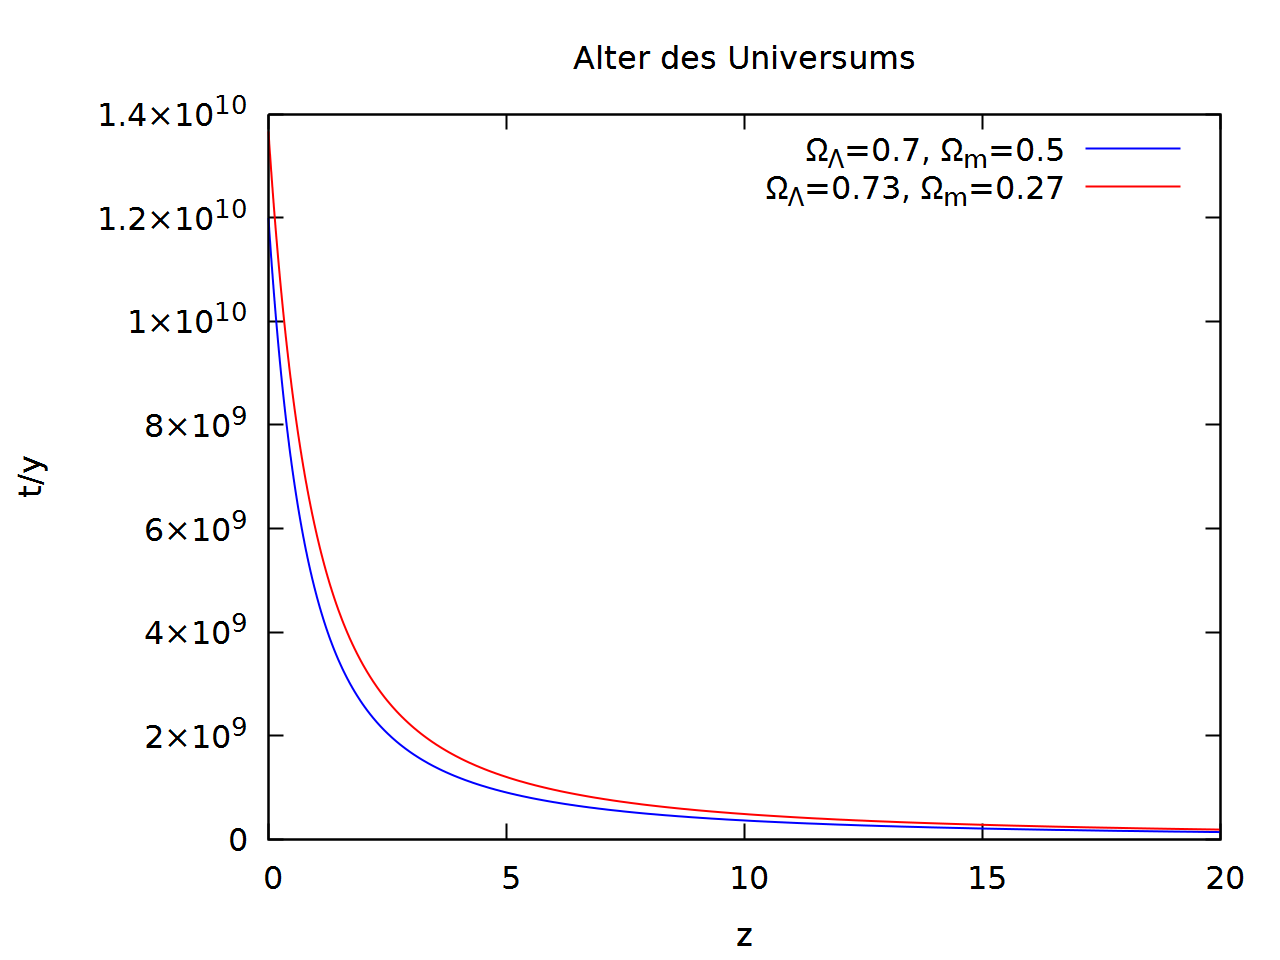
\includegraphics[scale=0.3]{plot_final} 
\captionof{figure}{Normaler Plot}
\end{center}
\begin{center}
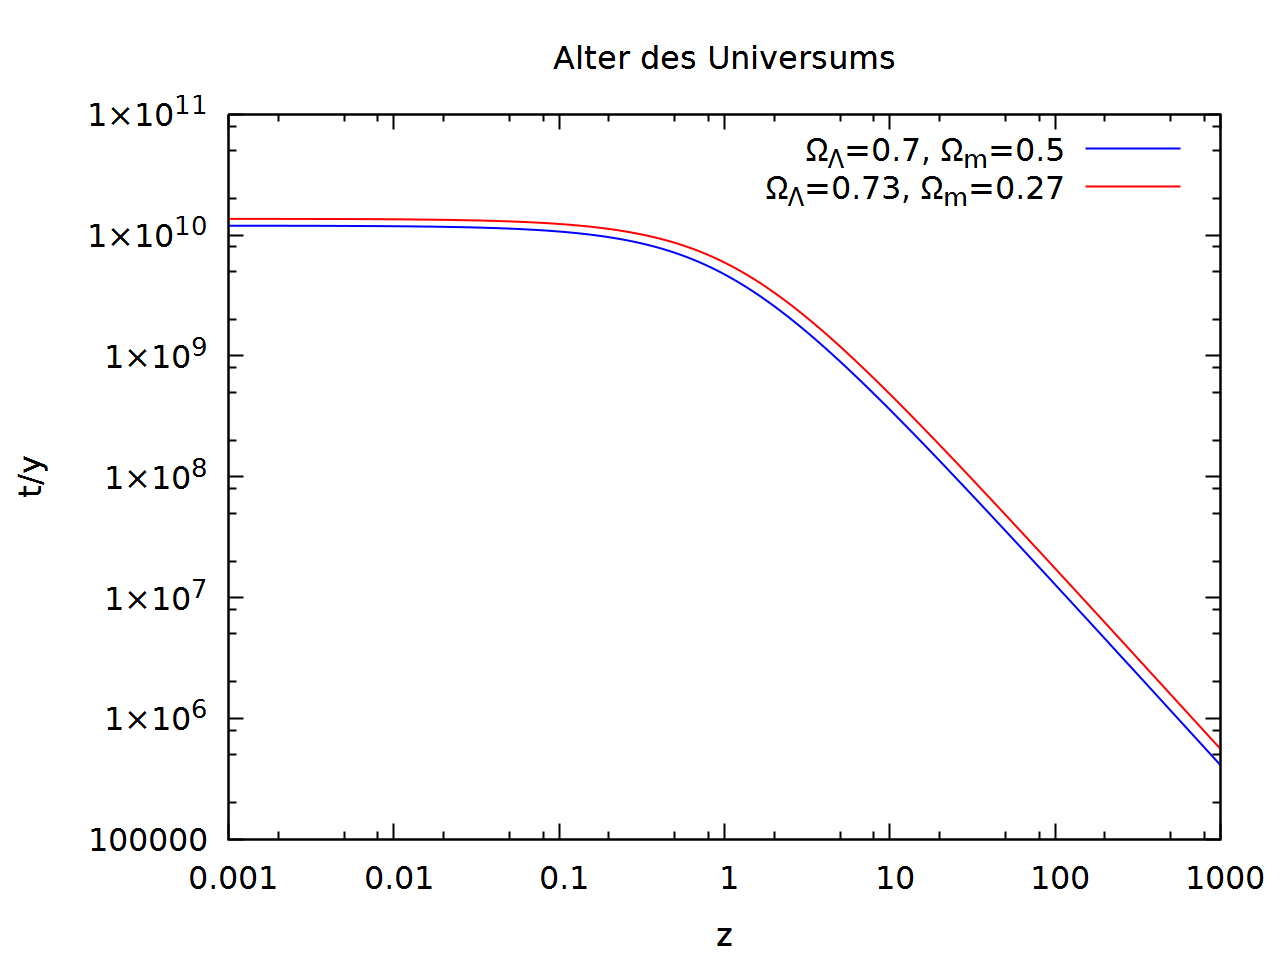
\includegraphics[scale=0.3]{plot_log_final} 
\captionof{figure}{Logarithmischer Plot}
\end{center}

\section*{Sonstige abgegebene Dateien}
\subsection*{plot\_final.plt}
Die Plot-Datei für die beiden Plots in der Abgabe.
\subsection*{b.txt}
Enthält die Plotdaten für b)
\subsection*{c.txt}
Enthält die Plotdaten für c)

\end{document}